\documentclass{article}
\usepackage[utf8]{inputenc}
\usepackage{amsmath,amsthm,amssymb,graphicx,mathtools,tikz,hyperref,enumerate, float}

\usepackage[
backend=biber,
style=numeric,
sorting=ynt
]{biblatex}
\addbibresource{ref.bib}

\title{CAI Classification Problem\\Report 1: Planning Phase}
\author{Nil Crespo-Peiró, Paco Rahn, Amin Ranem}
\date{12. January 2021}

\begin{document}

\maketitle

\section{Introduction}
This report covers the planning phase of the CAI Classification Problem. In the following section, an outline regarding the implementation of this project will be presented shortly. This planning includes the basic idea of how this project will be structured by the developers, given a Gantt Chart showing the defined deadlines for Prototypes and submissions. Lastly, the defined Network architecture provided at our initialised \href{https://github.com/amrane99/CAI-Classification/tree/main}{GitHub} repository will be briefly presented.

\section{Planning Phase}
In this section, the planning of the project will be presented, whereas the basic idea will be sketched in a first step, underpinned by a Gantt Chart representing the predefined deadlines for prototypes and further reports. Additionally, the implemented Network Architecture from our \href{https://github.com/amrane99/CAI-Classification/tree/main}{GitHub} repository so far will be described, followed by a representation of the \href{https://github.com/amrane99/CAI-Classification/tree/main}{repository}  directory structure in a final step.

\subsection{Sketch of the basic idea}
The main goal of our project is to implement a Deep Learning Method for tool detection in surgical operations. As in \cite{EndoNet} we will use a CNN and the \texttt{Cholec80} Dataset. Due to the lack of more data we want to use transfer learning and if the time allows it try out different network architectures. \\
\noindent
Furthermore, we will try to tackle the problem of small dataset by experimenting with data augmentation and dataset balancing.
As shown in \cite{EndoNet} the results from the tool detection task can be used as tool usage signals to perform phase recognition. With just two additional layers, a support vector machine and a hierarchical hidden markov network, Twinanda et al. were able to do tool detection and phase classification with the same network simultaneously. Depending on the results for the tool detection task we  consider to implement a phase classification as well.

\subsubsection{Gantt Chart}
Figure \ref{fig:gant} shows a Gantt chart with our plan for the next weeks. Beside the weekly tasks from the lecture we added some subtasks that we wish to accomplish. The list is not complete and some subtasks could be removed again.

\begin{figure}[htp!]
    \centering
    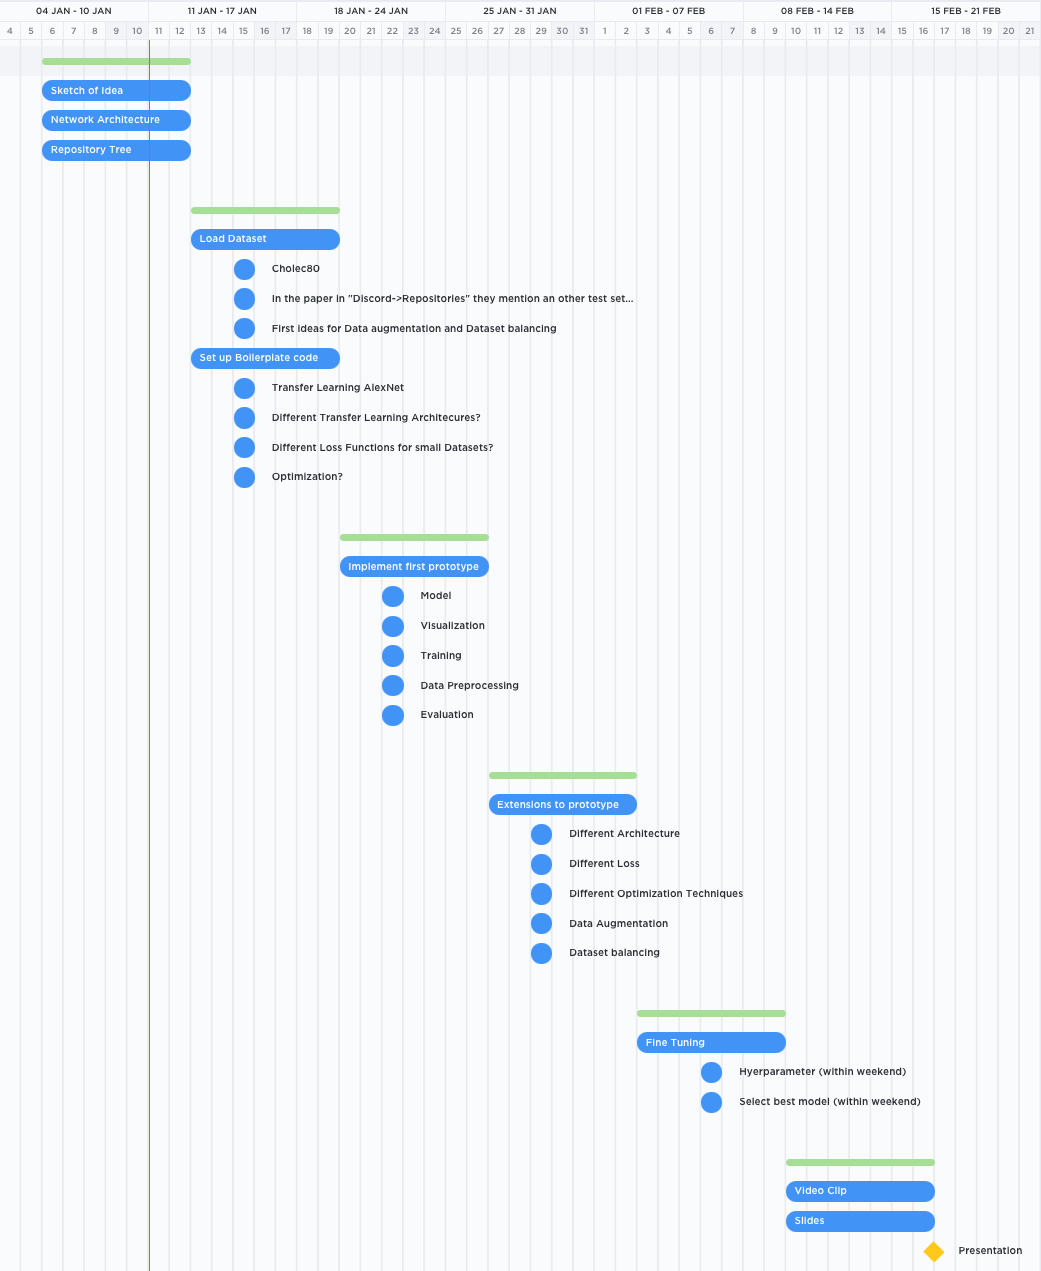
\includegraphics[width=\textwidth]{gant.png}
    \caption{Schedule for the Project}
    \label{fig:gant}
\end{figure}

\subsection{Network Architecture}

In this section we will be creating a tree graph in order to represent the network architecture of our GitHub Repository.\\
\noindent
In the first layer there are some documents of interest like the \texttt{README.md}, the \texttt{requirements.txt}, the \texttt{setup.py}, or the \texttt{code\_style\_conventions.py}, which ensure that everyone follows the same style while coding, states the requirements we will need to download in order to work in this project on how to set it all up before starting.\\ \\
\noindent
Then there are 3 major folders:
\begin{itemize}
    \item \texttt{docs}: A folder, where one can find the presentation, the video tutorial and the reports that have been created during the project.
    \item \texttt{test}: The folder in which the python tests will be saved in order to exclude as many bugs in our code as possible.
    \item \texttt{cai}: The main folder in which the structure of the data and the model itself will be defined, necessary functions for visualizations of the results will be saved and other important aspects like the GUI and the agent that trains the model.
\end{itemize}

\subsubsection{Directory tree structure of \href{https://github.com/amrane99/CAI-Classification/tree/main}{GitHub} repository}

\begin{figure}[H]
    \centering
    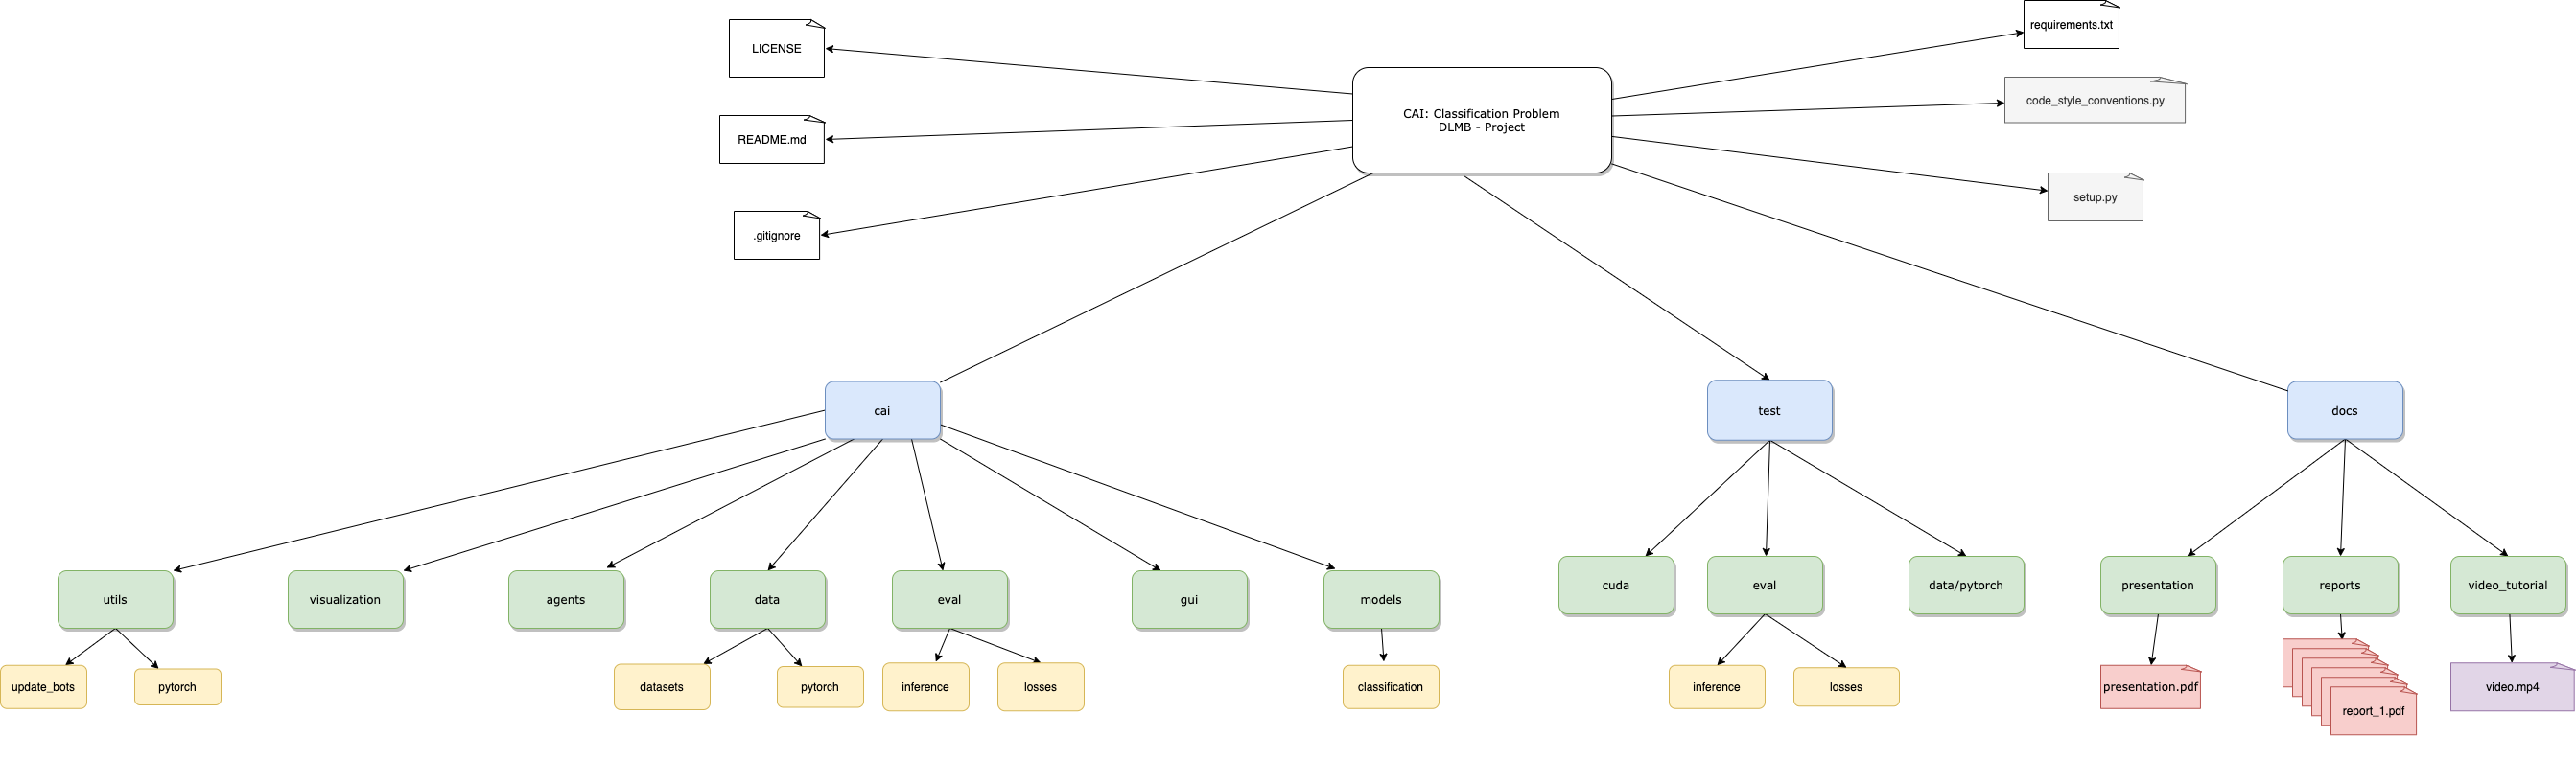
\includegraphics[width=\textwidth]{CAI diagram.png}
    \caption{Diagram of our GitHub Repository}
    \label{fig:diagram}
\end{figure}
\printbibliography
\end{document}